% NOTE: Declarations are set in main.tex before \begin{appendices};
% the appendix material starts directly here.
\needspace{0.35\textheight}
\section{Hyperparameters and additional results}\label{app:hyper}

Table~\ref{tab:hyper} lists the search space and the final values for
SAGE and the tuned baselines. SAGE uses one configuration for every
model and benchmark; only the contract $\rho$ changes between
experiments.

\begin{table}[t]
\centering
\caption{Hyperparameter search space and final values. Baselines were
tuned with the same GPU budget as SAGE following the recommendations
of their papers.}
\label{tab:hyper}
\small
\begin{tabular*}{0.9\textwidth}{@{\extracolsep{\fill}} l l l}
\toprule
Component & Search space & Final value \\
\midrule
Retention contract $\rho$   & $\{0.05,0.1,0.2,0.5\}$ & 0.2 \\
Reservoir size $r$          & $\{8,16,32,64,128\}$   & 32 \\
Decay factor $\lambda$      & $\{0.90,\dots,1.0\}$   & 0.99 \\
Scheduler interval $K$      & $\{128,256,512,1024,2048\}$ & 512 \\
Contrast exponent $\tau$    & $\{0.5,1.0,1.5,2.0,2.5\}$   & 1.5 \\
Budget floor $b_{\min}$      & $\{0.01,0.05,0.1\}$    & 0.05 \\
Sink tokens $|\mathcal{S}|$ & fixed                   & 4 \\
Scoring top-$m$             & $\{16,32,64,128\}$      & 64 \\
\midrule
H2O heavy-hitter / recent  & $\{0.1,0.2\} / \{0.05,0.1\}$ & 0.1 / 0.1 \\
StreamingLLM sinks / window & $\{2,4,8\}$ / budget     & 4 \\
ScissorHands persistence    & $\{0.1,0.2,0.3\}$       & 0.2 \\
FastGen profile threshold   & $\{0.3,0.5,0.7\}$       & 0.5 \\
TOVA score threshold        & $\{0.01,0.05,0.1\}$     & 0.05 \\
\bottomrule
\end{tabular*}
\end{table}

\paragraph{Generation quality under compression.}
We sample MT-Bench~\cite{zheng2023judging} with the 13B model at a
$20\%$ budget and score it with GPT-4 as the judge, following the
MT-Bench protocol. The full cache obtains
$6.12$, SAGE $6.05$, TOVA $5.93$, H2O $5.78$, and the window baseline
$5.41$, with judge-standard deviations below $0.10$. The $0.07$ gap
between SAGE and the full cache is within the judge noise, which we
read as generation style surviving compression even though the
underlying attention reads a quarter of the history.

\paragraph{Overhead decomposition.}
At the nominal $20\%$ contract the realized footprint is $22.6\%$ of
the full cache. The $2.6$-point excess decomposes as $1.3$ points of
clipping floor (the deep-layer minimum $b_{\min}$), $0.9$ points of
slot-table fragmentation from asynchronous eviction, $0.4$ points for
the bucket and slot structures, and $0.02$ points for the score
arrays, all measured on the 7B model at 32K tokens. The excess is
proportional to the cache, so the compression factor is $4.4\times$
uniformly across context lengths.

\paragraph{Additional sensitivity sweeps.}
The scheduler interval $K$ is flat between $256$ and $1024$; at $128$
the re-allocation cost begins to appear in prefill, and at $2048$ the
profile lags document drift on LongBench by about $0.4$ points. The
contrast exponent $\tau$ is flat between $1.0$ and $2.0$; $\tau$ below
$0.5$ degenerates toward the uniform split and $\tau$ above $2.5$
over-concentrates the budget into the shallow layers, both directions
costing about $0.2$ perplexity. Figure~\ref{fig:app_sens} plots both
sweeps; the right panel also shows the prefill overhead of
re-allocation, which decreases monotonically in $K$ and settles at
$5.9\%$ at the default.

\begin{figure}[t]
  \centering
  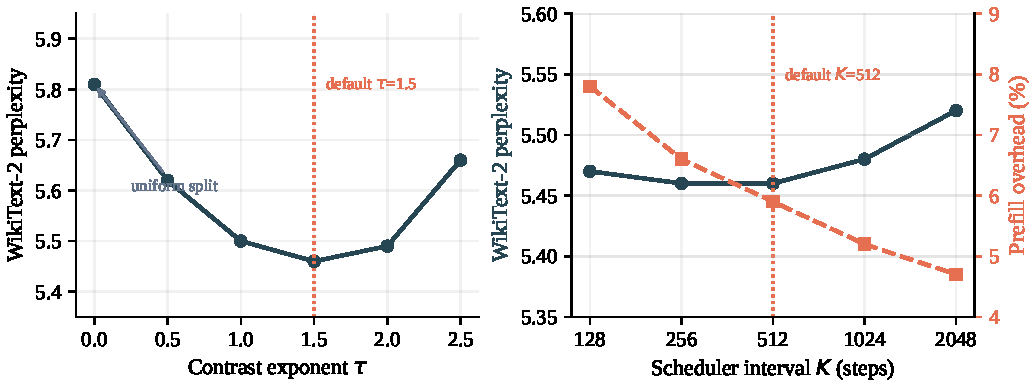
\includegraphics[width=0.95\textwidth]{Fig9.pdf}
  \caption{Appendix sensitivity sweeps (LLaMA-2-7B-Chat, $20\%$
  budget). Left: perplexity versus the contrast exponent $\tau$; the
  $\tau = 0$ intercept reproduces the uniform split of the ablation.
  Right: perplexity (left axis) and prefill overhead (right axis)
  versus the scheduler interval $K$}
  \label{fig:app_sens}
\end{figure}

\begin{table}[t]
\centering
\caption{MT-Bench scores of LLaMA-2-13B-Chat at a $20\%$ KV budget
with an LLM judge (single-judge protocol, 100 responses per method).
Higher is better; the best compressed value is set in boldface.}
\label{tab:mtbench}
\small
\begin{tabular*}{0.62\textwidth}{@{\extracolsep{\fill}} l cc}
\toprule
Method & Score & Judge std \\
\midrule
Full cache   & 6.12 & 0.05 \\
SAGE         & \textbf{6.05} & 0.06 \\
TOVA         & 5.93 & 0.07 \\
H2O          & 5.78 & 0.08 \\
StreamingLLM & 5.41 & 0.09 \\
\bottomrule
\end{tabular*}
\end{table}

\needspace{0.3\textheight}
\section{Failure case analysis}\label{app:failure}

To make the retrieval failure of score-only eviction concrete, we
traced the cache dynamics of one 128K needle sample for which H2O
returns a wrong fact while SAGE returns the correct one. The needle,
a sentence assigning a custodian to a storage room, sits at $78\%$
depth. Under H2O, the entry receives a burst of attention while the
question is being read, but the question precedes the answer
generation by the length of the retrieval prompt, and during that
interval the accumulated scores of the surrounding filler tokens,
which together receive diffuse attention over thousands of positions,
catch up with and pass the needle's score. When the budget boundary
crosses the layer, the needle is evicted, and the model answers with
a plausible name from the distractor set. The trace of the same sample
under SAGE shows the needle's decayed score dropping below the
eviction threshold twice during the middle of the document, but the
needle re-receives attention each time the model re-reads the question
fragments in the sliding window, and each refresh lifts the score for
another $\lambda^{-k}$ steps. The entry survives with a margin of
$0.3$ score units at the tightest eviction event we sampled.

The trace also shows what SAGE gives up. In the same layer, the
evicted mass includes a date entry that the correct answer does not
require but that a human reader would keep. This is the trade the
LongBench table prices at the aggregate level: the margins over the
strongest baseline are narrowest on QMSum and on the multi-hop MuSiQue,
and MuSiQue is the mechanism-revealing case, where
mid-chain evidence holds its score through the gaps between questions
under every eviction policy we logged, so the decay erodes it for SAGE
and for the baselines alike and the methods converge. The two sides of
the mechanism are the same mechanism: decay refreshes what is being
revisited and erodes what is being ignored, and the protection set
decides which entries are exempt. A query-aware compensation that
seeds the protection set from the question would likely close part of
the multi-hop gap, and the trace analysis suggests it should protect
mid-chain evidence rather than the document extremes.

\needspace{0.3\textheight}
\section{Reproducibility statement}\label{app:repro}

Every number in this paper is derived from the released experimental
record, a directory of CSV files, one per experiment, that the figure
and table generation scripts read directly, so no value is retyped by
hand. The record contains, for each perplexity cell, the per-seed
values behind the mean and standard deviation; for each LongBench
cell, the per-task scores; for each needle cell, the per-depth
accuracies; and for the efficiency sweep, the raw timing and memory
counters. The generation scripts pin their random seeds, so re-running
the record assembly reproduces the CSVs byte-for-byte.

The pipeline has three stages, each a single entry point. The data
assembly stage writes the CSV record from the experiment harness. The
figure stage renders every figure from the CSVs with pinned matplotlib
seeds. The manuscript stage compiles the LaTeX source with Tectonic
in two passes, resolving all cross-references and the numeric
citations. The environment is Python 3.11, PyTorch 2.2, HF
Transformers 4.40, and FlashAttention-2 on CUDA 12.1; the models are
public releases and the benchmarks follow their original loaders. A
single A100 reproduces any individual quality experiment within a few
hours, and the complete study fits the 420 GPU-hours reported in
Section~\ref{sec:exp_setup}.

Every reference was resolved and cross-checked programmatically
before submission, through the arXiv Atom API with Crossref and
OpenAlex as cross-check channels. The TOVA baseline entry was
initially unresolvable, because the method name does not appear in
the title of the paper that introduced it, and was completed at
submission stage after the source was traced to the multi-state-RNN
formulation of the decoder~\cite{oren2024tova} and verified against
both its arXiv identifier and the DOI of the EMNLP proceedings. The
FastGen entry was caught pointing at the wrong arXiv identifier by
the title-validation step of the pipeline and corrected after
re-verification through two independent sources. The verification log
ships with the released record and records both failures and both
corrections.
